\documentclass[12pt,twoside]{report}

%%%%%%%%%%%%%%%%%%%%%%%%%%%%%%%%%%%%%%%%%%%%%%%%%%%%%%%%%%%%%%%%%%%%%%%%%%%%%

% Definitions for the title page
% Edit these to provide the correct information
% e.g. \newcommand{\reportauthor}{Timothy Kimber}

\newcommand{\reporttitle}{Title}
\newcommand{\reportauthor}{Luca Grillotti}
\newcommand{\supervisor}{Krysia Broda}
\newcommand{\degreetype}{Computing Science / Artificial Intelligence}

%%%%%%%%%%%%%%%%%%%%%%%%%%%%%%%%%%%%%%%%%%%%%%%%%%%%%%%%%%%%%%%%%%%%%%%%%%%%%

% load some definitions and default packages
%%%%%%%%%%%%%%%%%%%%%%%%%%%%%%%%%%%%%%%%%
% University Assignment Title Page 
% LaTeX Template
% Version 1.0 (27/12/12)
%
% This template has been downloaded from:
% http://www.LaTeXTemplates.com
%
% Original author:
% WikiBooks (http://en.wikibooks.org/wiki/LaTeX/Title_Creation)
%
% License:
% CC BY-NC-SA 3.0 (http://creativecommons.org/licenses/by-nc-sa/3.0/)
% 
%
%%%%%%%%%%%%%%%%%%%%%%%%%%%%%%%%%%%%%%%%%
%----------------------------------------------------------------------------------------
%	PACKAGES AND OTHER DOCUMENT CONFIGURATIONS
%----------------------------------------------------------------------------------------
\usepackage[a4paper,hmargin=2.8cm,vmargin=2.0cm,includeheadfoot]{geometry}
\usepackage{textpos}
\usepackage{natbib} % for bibliography
\usepackage{tabularx,longtable,multirow,subfigure,caption}%hangcaption
\usepackage{fncylab} %formatting of labels
\usepackage{fancyhdr} % page layout
\usepackage{url} % URLs
\usepackage[english]{babel}
%\usepackage{svg}
\usepackage{amsmath}
\usepackage{appendix}
\usepackage{graphicx}
\usepackage{dsfont}
\usepackage{epstopdf} % automatically replace .eps with .pdf in graphics
\usepackage{backref} % needed for citations
\usepackage{array}
\usepackage{latexsym}
\usepackage[pdftex,pagebackref,hypertexnames=false,colorlinks]{hyperref} % provide links in pdf
\usepackage{makecell}
\usepackage{fancyvrb}
\usepackage{color}
\usepackage[dvipsnames]{xcolor}


\hypersetup{pdftitle={},
  pdfsubject={}, 
  pdfauthor={},
  pdfkeywords={}, 
  pdfstartview=FitH,
  pdfpagemode={UseOutlines},% None, FullScreen, UseOutlines
  bookmarksnumbered=true, bookmarksopen=true, colorlinks,
    citecolor=black,%
    filecolor=black,%
    linkcolor=black,%
    urlcolor=black}

\usepackage[all]{hypcap}

\usepackage{amsthm}
\usepackage{verbatim}
\theoremstyle{definition}

%\usepackage{color}
%\usepackage[tight,ugly]{units}
%\usepackage{float}
%\usepackage{tcolorbox}
%\usepackage[colorinlistoftodos]{todonotes}
% \usepackage{ntheorem}
% \theoremstyle{break}
\newtheorem{lemma}{Lemma}[section]
\newtheorem{theorem}{Theorem}[section]
\newtheorem{remark}{Remark}
\newtheorem{definition}{Definition}[section]
% \newtheorem{proof}{Proof}


%%% Default fonts
\renewcommand*{\rmdefault}{bch}
\renewcommand*{\ttdefault}{cmtt}


%%% Default settings (page layout)
\setlength{\parindent}{0em}  % indentation of paragraph

\setlength{\headheight}{14.5pt}
\pagestyle{fancy}
\renewcommand{\chaptermark}[1]{\markboth{\chaptername\ \thechapter.\ #1}{}} 

\fancyfoot[ER,OL]{\sffamily\textbf{\thepage}}%Page no. in the left on odd pages and on right on even pages
\fancyfoot[OC,EC]{\sffamily }
\renewcommand{\headrulewidth}{0.1pt}
\renewcommand{\footrulewidth}{0.1pt}
\captionsetup{margin=10pt,font=small,labelfont=bf}


%--- chapter heading

\def\@makechapterhead#1{%
  \vspace*{10\p@}%
  {\parindent \z@ \raggedright \sffamily
    \interlinepenalty\@M
    \Huge\bfseries \thechapter \space\space #1\par\nobreak
    \vskip 30\p@
  }}

%---chapter heading for \chapter*  
\def\@makeschapterhead#1{%
  \vspace*{10\p@}%
  {\parindent \z@ \raggedright
    \sffamily
    \interlinepenalty\@M
    \Huge \bfseries  #1\par\nobreak
    \vskip 30\p@
  }}

\allowdisplaybreaks



% load some macros
% Here, you can define your own macros. Some examples are given below.

\newcommand{\R}[0]{\mathds{R}} % real numbers
\newcommand{\Z}[0]{\mathds{Z}} % integers
\newcommand{\N}[0]{\mathds{N}} % natural numbers
\newcommand{\C}[0]{\mathds{C}} % complex numbers
\renewcommand{\vec}[1]{{\boldsymbol{{#1}}}} % vector
\newcommand{\mat}[1]{{\boldsymbol{{#1}}}} % matrix


\date{September 2015}

\begin{document}

% load title page
% Last modification: 2015-08-17 (Marc Deisenroth)
\begin{titlepage}

\newcommand{\HRule}{\rule{\linewidth}{0.5mm}} % Defines a new command for the horizontal lines, change thickness here


%----------------------------------------------------------------------------------------
%	LOGO SECTION
%----------------------------------------------------------------------------------------


\includegraphics[width = 4cm]{./figures/imperial}\\[0.5cm] 

\center % Center remainder of the page

%----------------------------------------------------------------------------------------
%	HEADING SECTIONS
%----------------------------------------------------------------------------------------

\textsc{\Large Imperial College London}\\[0.5cm] 
\textsc{\large Department of Computing}\\[0.5cm] 

%----------------------------------------------------------------------------------------
%	TITLE SECTION
%----------------------------------------------------------------------------------------

\HRule \\[0.4cm]
{ \huge \bfseries \reporttitle}\\ % Title of your document
\HRule \\[1.5cm]
 
%----------------------------------------------------------------------------------------
%	AUTHOR SECTION
%----------------------------------------------------------------------------------------

\begin{minipage}{0.4\textwidth}
\begin{flushleft} \large
\emph{Author:}\\
\reportauthor % Your name
\end{flushleft}
\end{minipage}
~
\begin{minipage}{0.4\textwidth}
\begin{flushright} \large
\emph{Supervisor:} \\
\supervisor % Supervisor's Name
\end{flushright}
\end{minipage}\\[4cm]


%----------------------------------------------------------------------------------------
%	FOOTER & DATE SECTION
%----------------------------------------------------------------------------------------
\vfill % Fill the rest of the page with whitespace
Submitted in partial fulfillment of the requirements for the MSc degree in
\degreetype~of Imperial College London\\[0.5cm]

\makeatletter
\@date 
\makeatother


\end{titlepage}



% page numbering etc.
\pagenumbering{roman}
\clearpage{\pagestyle{empty}\cleardoublepage}
\setcounter{page}{1}
\pagestyle{fancy}

%%%%%%%%%%%%%%%%%%%%%%%%%%%%%%%%%%%%
\begin{abstract}
Your abstract.
\end{abstract}

\cleardoublepage
%%%%%%%%%%%%%%%%%%%%%%%%%%%%%%%%%%%%
%*%\section*{Acknowledgments}
%*%Comment this out if not needed.

\clearpage{\pagestyle{empty}\cleardoublepage}

%%%%%%%%%%%%%%%%%%%%%%%%%%%%%%%%%%%%
%--- table of contents
\fancyhead[RE,LO]{\sffamily {Table of Contents}}
\tableofcontents 


\clearpage{\pagestyle{empty}\cleardoublepage}
\pagenumbering{arabic}
\setcounter{page}{1}
\fancyhead[LE,RO]{\slshape \rightmark}
\fancyhead[LO,RE]{\slshape \leftmark}

%%%%%%%%%%%%%%%%%%%%%%%%%%%%%%%%%%%%
%*%\chapter{Introduction}
%%%%%%%%%%%%%%%%%%%%%%%%%%%%%%%%%%%%
\chapter{Background}

\section{Answer Set Programming (ASP)}

\subsection{Logic Program}

We will work on finite Logic Programs with rules of the form:
\begin{itemize}
\item $\leftarrow b_1, b_2, ..., b_m, \text{ not } c_1, \text{ not } c_2,...,\text{ not } c_n$ (also called \textit{constraint}).
\item $a \leftarrow b_1, b_2, ..., b_m, \text{ not } c_1, \text{ not } c_2,...,\text{ not } c_n$. This is a \textit{default} rule.
\item $l\{a_1, a_2, ..., a_p\}u \leftarrow b_1, b_2, ..., b_m, \text{ not } c_1, \text{ not } c_2,...,\text{ not } c_n$, where $l$ and $u$ are numbers such that $l \leq u$. Also, $l\{a_1, a_2, ..., a_p\}u$ is true in an Herbrand Interpretation $I$ iff $ l \leq |\{a_1, a_2, ..., a_p\}\cap I | \leq u$. This type of rule is also called \textit{choice rule}.
\end{itemize}
In all these rules, "$\text{ not }$" refers to the \textit{"negation as failure"}, and $a, a_1, a_2, ..., a_p, b_1, b_2,\\ ..., b_m, c_1, c_2, ...,  c_n$ are atoms. 

\smallskip

$a$ and $l\{a_1, a_2, ..., a_p\}u$ are called the \textit{head} of the rule, and $b_1, b_2, ..., b_m, \text{ not } c_1, \text{ not } c_2,\\..., \text{ not } c_n$ is the \textit{body} of the rule. If we call $r$ the following rule: $\alpha \leftarrow b_1, b_2, ..., b_m,\\ \text{ not } c_1, \text{ not } c_2,...,\text{ not } c_n$ where $\alpha$ is either an atom or an aggregate, then $body^+(r)=\{b_1, b_2,...,b_m \}$ and $body^-(r)=\{c_1, c_2,...,c_n \}$.

\smallskip

A \textit{literal} is an atom or the negation (by failure) of an atom.

\subsection{Stable Models (Answer Sets)}

Let $P$ be a logic program and $X$ be an Herbrand Interpretation of $P$. From $P$ and $X$, we can construct a new program $P^X$ called the \textit{reduct} of $P$ by applying these methods:
\begin{itemize}
\item For every rule $r\in P$, if $X\cap body^-(r)=\emptyset$, then we remove every negative literal in $r$.
\item Otherwise, if $X\cap body^-(r)\neq\emptyset$, then we delete the whole rule.
\item We replace every constraint $ :- body$ by $\perp :- body$. Here $\perp$ is an atom that does not appear in $P$. As a consequence, $\perp$ does not belong to any Answer Set.
\item For every rule $r$ with an aggregate in the head: $l\{a_1, a_2, ..., a_p\}u \leftarrow b_1, b_2, ..., b_m$ (we suppose that we have already removed the negative literals according to the first method)
\begin{itemize}
\item if $l \leq |\{a_1, a_2, ..., a_p\}\cap X | \leq u$, we replace $r$ by all the rules in the following set: $\{ a_i \leftarrow b_1, b_2, ..., b_m | a_i \in X\}$.
\item otherwise, we replace $r$ by $\perp \leftarrow b_1, b_2, ..., b_m$
\end{itemize}
\end{itemize}

Thus, the reduct $P^X$ is a \textit{definite} logic program (which means that it does not contain any negation as failure). Definite logic programs have a unique minimal Herbrand model, that is very easy to construct. We will write $M(P^X)$ the minimal Herbrand model of $P_X$.

\smallskip

We call \textit{stable model} of $P$ every Herbrand interpretation $X$ that satisfies the relation: $X=M(P^X)$. Moreover, as we do not use classical negation $\neg$, we will not make a distinction between \textit{answer sets} and stable models.

\smallskip

Stable models of $P$ have more properties than its models in general: they also are \textit{minimal} (for inclusion) and \textit{supported} (every atom in the stable model appears in a rule whose body evaluates to \textit{true}). 

\subsection{Tools}

For ASP problems, we will use some of the tools developed by the University of Potsdam: \texttt{gringo}, \texttt{clasp} and \texttt{clingo}. \texttt{gringo} transforms the logic program in input into an equivalent variable-free program (it is a \textit{grounder}). And \texttt{clasp} is a \textit{solver} capable of solving ground logic programs. Finally, \texttt{clingo} only combines grounding (with \texttt{gringo}) and solving (with \texttt{clasp}).
%TODO : reference manuel
\section{Single-Player Games in ASP}

It is possible to formalize and solve Single-Player Games in ASP. To illustrate the predicates that can be used to describe these games, we will focus on a basic example: a simple graph game.

%TODO : référence 

\subsection{Rules of the game}

The rules of the graph game on figure \ref{fig:agent} are the following:
\begin{itemize}
\item The player starts in state $a$.
\item If the player is in state $a$ or in state $b$ then he can go to the left or to the right.
\item The player wins iff he goes to the state \textit{"victory"}.
\item The player cannot go back to state $a$ once he has reached the state \textit{"hole"}.
\end{itemize}

\begin{figure}[h]
\centering
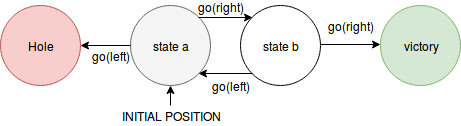
\includegraphics[width = 0.8\hsize]{diagram1.png}
\caption{Simple graph game}
\label{fig:agent}
\end{figure}

\subsection{Formalizing these rules}

\begin{itemize}



\item We start by defining the different players in the game by using the predicate \texttt{role}. Here, there is only one player so we include the fact: \texttt{role(player).}

\smallskip

\item Then, we define what are the initial states by using the predicate \texttt{holds} for the first time-step:\newline
\texttt{holds(hole, empty, 1).}\\
\texttt{holds(a, player, 1).} \% the player is in state $a$\\
\texttt{holds(b, empty, 1).}\\
\texttt{holds(victory, empty, 1).}

\item We also say what actions are legal at time $T$, depending on the state the player is:\newline
\texttt{legal(player,go(left),T) :- holds(a,player,T) ; holds(b,player, T)}\\
\texttt{legal(player,go(right),T) :- holds(a,player,T) ; holds(b,player,T)}

\item And we explain the situation at time $T+1$ depends on what holds at time $T$ and what the player does:\newline
\texttt{holds(hole,player,T+1) :- holds(a,player,T), does(player,go(left),T).}\\
\texttt{holds(b,player,T+1) :- holds(a,player,T), does(player,go(right),T).}\\
\texttt{...}

\item We can also define what is a \texttt{terminal} state, and we can evaluate each final state by using the predicate \texttt{goal}: \newline
\texttt{terminal(T) :- holds(victory, player, T).}\\
\texttt{terminal(T) :- holds(hole, player, T).}\\
\texttt{goal(player,100,T) :- holds(victory, player, T).}\\
\texttt{goal(player,  0,T) :- holds(hole, player, T).}
\end{itemize}

We will follow the following Game Description Language (GDL) restriction: the predicate \texttt{does} does not appear in the definition of \texttt{terminal}, \texttt{goal} or \texttt{legal}. Also, \texttt{does} only appears in rule bodies. 

\subsection{Finding a solution to the game}

We have just defined a few predicates to translate the rules of the game in ASP. Now we want to simulate the game and to find winning sequences of moves.
\begin{itemize}
\item First of all, the player can do only one move at every time step (as long as the game is not finished).\newline
\texttt{1\{does(player,go(left),T);does(player,go(right),T)\}1 :- not terminated(T).}\\
Where \texttt{terminated(T)} is true if and only if there is a T1 such that $T1<T$ and \texttt{terminal(T1)} is true:\newline
\texttt{terminated(T) :- terminal(T).}  \\
\texttt{terminated(T+1) :- terminated(T).}

\item Also, every move that is played must be legal:\newline
\texttt{:- does(player, M, T), not legal(player, M, T).}

\item We want the game to terminate at some point:\newline
\texttt{:- 0\{terminated(T) : time\_domain(T)\}0.}\\
\texttt{time\_domain(1..10). \% We allow at most 10 moves} 

\item 

\end{itemize}



\section{Inductive Logic Programming}

In this part, $B$ is the logic program that represents the \textit{Background Knowledge}, $S_M$ is the set of possible hypotheses, $E^+$ is the set of positive examples (all the elements that have been observed) and $E^-$ is the set of negative examples (all the elements that can't appear in any result). Our task is to find an hypothesis $H\in S_M$ such that $B\cup H$ \textit{explains} $E^+$ and $E^-$. There are different ways of defining the word "explains" used in the last sentence. We will have a look at three of them.

%TODO S_M ???

\subsection{Brave Inductive Logic Programming}

\subsubsection{Brave Induction}

A brave inductive task is a tuple $T_b=<B, E^+, E^->$ (where $E^+$ and $E^-$ are sets of atoms occurring in $B$) such that: an hypothesis $H$ is solution of $T_b$ iff there is an answer set $A$ of $B\cup H$ verifying $E^+\subseteq A$ and $E^-\cap A = \emptyset$

\smallskip

We call $ILP_b(B,E^+,E^-)$ the set of hypotheses that are solutions of $T_b$. 

\subsubsection{ASPAL encoding}

%TODO défauts d'ASPAL

\subsection{Cautious Inductive Logic Programming}

A cautious inductive task is a tuple $T_c=<B, E^+, E^->$ (where $E^+$ and $E^-$ are sets of atoms occurring in $B$) such that: an hypothesis $H$ is solution of $T_c$ iff 
\begin{itemize}
\item $B\cup H$ has at least one answer set
\item every answer set of $B\cup H$ verifies $E^+\subseteq A$ and $E^-\cap A = \emptyset$
\end{itemize}

We call $ILP_c(B,E^+,E^-)$ the set of hypotheses that are solutions of $T_c$. 

%TODO pas possible avec clingo

\subsection{Inductive Learning From Answer Sets Programming}

We present here a new type of inductive task which is more general than the cautious and the brave inductive tasks.

\subsubsection{Partial Interpretations}

We call \textit{partial interpretation} a tuple $<e^+,e^->$ where $e^+=\{e^+_1,e^+_2,...,e^+_m\}$ and $e^-=\{e^-_1,e^-_2,...,e^-_n\}$ are two sets of atoms.

\smallskip

We say that an interpretation $I$ of $B$ extends a partial interpretation $<e^+,e^->$ iff $e^+ \subseteq I$ and $e^- \cap I = \emptyset$.

\subsubsection{Learning from Answer Sets Induction}

A Learning from Answer Sets task is a tuple $T_{LAS}=<B, S_M, E^+, E^->$ (where $E^+$ and $E^-$ are sets of partial interpretations) such that: an hypothesis $H$ is solution of $T_{LAS}$ iff 
\begin{itemize}
\item For all  $<e^+,e^->\in E^+$, there is an answer set of $B\cup H$ that extends $<e^+,e^->$
\item For all  $<e^+,e^->\in E^-$, there are no answer sets of $B\cup H$ that extend $<e^+,e^->$
\end{itemize}

We call $ILP_{LAS}(B,S_M,E^+,E^-)$ the set of hypotheses that are solutions of $T_{LAS}$. 

\subsubsection{ILASP}

ILASP is a tool developed at Imperial College London that is capable of finding optimal hypotheses for Learning from Answer Sets tasks. We only need to give it: the background knowledge with the \texttt{clingo} syntax, and the mode declaration for the variables that can appear in the head or in the body of a rule in the hypothesis. We can also specify the positive and negative partial interpretations of the task.

\begin{itemize}
\item Learning from Answer Sets Induction
\item ILASP
\begin{itemize}
\item examples of what has been done so far
\item learning weak constraints ?
\item contexts
\item noisy examples
\end{itemize}
\end{itemize}

%%%%%%%%%%%%%%%%%%%%%%%%%%%%%%%%%%%%
\chapter{Progress}

\section{Two-Players games}

\subsection{Representing Two-Players games in ASP}

We only need to change a few things to adapt the rules in single-player games for two-players games:
\begin{itemize}
\item First of all, we create two roles instead of one:\\ \texttt{role(player1).}\\
\texttt{role(player2).}
\item Then we replace \texttt{player} in every rule by the variable \texttt{P}, and we add \texttt{role(P)} at the end of each rule.
\item Besides, only one move is allowed at each time step:\\
\texttt{1\{does(P,M,T):role(P),move\_domain(M)\}1 :- not terminated(T).}\\
\texttt{move\_domain(go(left))}.\\
\texttt{move\_domain(go(right))}.

\item Finally, a player cannot play twice:\\
\texttt{:- does(P,M1,T), does(P,M2,T+1).}

\end{itemize}

\subsection{Games under study}

This project focuses on three games: \textit{Five Field Kono}, \textit{Nine Men's Morris} and \textit{ASALTO}.

%TODO : give references

\smallskip

For the moment, we have only tried to study how to learn a strategy on a very simple game (with a small number of possible states): the \textit{tic-tac-toe}. Afterwards, we will try to extend what we have done on \textit{tic-tac-toe} to \textit{Five Field Kono}.

\smallskip

Moreover, we have represented these four games in ASP.

\section{Finding/Learning a strategy}

We found several ways of thinking about how to learn a strategy:
\begin{itemize}
\item The first one consists in trying to find a move such that: whatever the second player does the next turn (or his 2 or 3 next turns), the first player can still win. This method seems very similar to the \textit{minimax} algorithm. 
\item We could also study several games played by two players, and try to make hypotheses about what to do in which circumstances. 
\item It is possible to imagine a mix between the two previous methods: the second one tells us what are the good states, and the first method gives us a move so that we can reach a good state for sure (whatever the second player does).
\end{itemize}

For the moment, we have only studied the first method.

%TODO : give references (minimax)
%TODO : parler des inconvénients de chaque méthode.

\subsection{Planning moves}

\subsubsection{Basic method}

In \textit{tic-tac-toe}, we initialized the game with 4 specific moves already done. If we restrict the hypothesis space by not allowing negation by failure nor constraints, ILASP can find some (ground) hypotheses of the form:\\
\texttt{does(player1,fill(cell(x)),5). \% at time T=5 } \\
\texttt{does(player1,fill(cell(y)),7) :- does(player2,fill(cell(z)),6).}\\
that make \texttt{player1} win. 

\smallskip

For this, we only need to specify that the program has at least an answer set: \texttt{\#pos(\{\},\{\})}, and that \texttt{player1} wins in every answer set: \texttt{\#neg(\{\},\{wins(player1)\})}.

\subsubsection{Problem with negation by failure}



\subsubsection{Solution Found for the Graph Games}



%%%%%%%%%%%%%%%%%%%%%%%%%%%%%%%%%%%%
%*%\chapter{Experimental Results}


%%%%%%%%%%%%%%%%%%%%%%%%%%%%%%%%%%%%
\chapter{Implementation}

For the moment, we only have implemented the \textit{tic-tac-toe} and the \textit{Field Field Kono} in python by using \texttt{pygame} (python library for video games).
%TODO : reference pygame
\smallskip

The idea would be to learn from the actions performed by a player to train our system by using ILASP. Then we could make him play against this trained system and continue to train it that way.

\section{First Method: maximize the chances of winning}
%TODO : Change title ?

\subsection{Learning Exception Structure}

Supposing we are at time $T=t$, we want the computer to induce a set of rules $H$ such that:
\begin{itemize}
\item There is a move $m$ such that for every answer set $A$ of $B\cup H,\:  does(player1, m, t)\in A$
\item For every answer set $A$ of $B\cup H$, for all move $m_1$ different from $m$, we have: $does(player1, m_1, t) \notin A$
\item $H$ also tries to take into account the possible future moves.
\end{itemize}

To reduce the hypothesis space, it would be interesting to focus only on \textit{exception structures}, which means we want $H$ to be of this form:
\[H=
\begin{Bmatrix}
\texttt{does(player1, move\_p1\_t0\_1, t).}\\
\texttt{does(player1, move\_p1\_t2\_1, t+2) :- \textcolor{red}{does(player2, move\_p2\_t1\_1, t+1)}.}\\
\texttt{does(player1, move\_p1\_t2\_2, t+2) :- not \textcolor{red}{does(player2, move\_p2\_t1\_1, t+1)}.} 
\end{Bmatrix}
\]
%TODO : A FAIRE avec le cours de Marek Sergot ???
In the set above, we will call "\textit{exception rule}" the second rule, and "\textit{general rule}" the third.

\begin{remark}
 The hypothesis space could also be extended so that it accepts two or more  exception rules.
\[H=
\begin{Bmatrix}
\texttt{does(player1, move\_p1\_t0\_1, t).}\\
\texttt{does(player1, move\_p1\_t2\_1, t+2) :-} &\texttt{\textcolor{red}{does(player2, move\_p2\_t1\_1, t+1)}.}\\
\texttt{does(player1, move\_p1\_t2\_2, t+2) :-} &\texttt{\textcolor{blue}{does(player2, move\_p2\_t1\_2, t+1)}.}\\
\texttt{does(player1, move\_p1\_t2\_3, t+2) :-} &\texttt{not \textcolor{red}{does(player2, move\_p2\_t1\_1, t+1)},}\\ &\texttt{not \textcolor{blue}{does(player2, move\_p2\_t1\_2, t+1)}.} 
\end{Bmatrix}
\]
\end{remark}

%TODO : Deuxième remarque pour expliquer comment prendre en compte ce qu'il se passe à t+4 ?

Moreover, the atoms in the exception rule must appear in the general rule (see the \textcolor{red}{red} and \textcolor{blue}{blue} atoms in the hypotheses above).

\bigskip

%TODO : good version of ILASP ?
With ILASP 3.1.0 it is possible add "bias constraints" to specify what kind of rule we want to learn. However it is not possible to add constraints on the whole set of rules induced. As a consequence, we cannot say that for every solution $H$ in $ILP_{LAS}(B,S_M,E^+,E^-)$, 
if there are $move\_p1\_t2\_1$ and $move\_p2\_t1\_1$ such that:
\\ $\texttt{"does(player1,move\_p1\_t2\_1,t+2) :- \textcolor{red}{does(player2,move\_p2\_t1\_1,t+1)}."}\in H$, 
then there is $move\_p1\_t2\_2$ such that:\\
$\texttt{"does(player1,move\_p1\_t2\_2,t+2):- not \textcolor{red}{does(player2,move\_p2\_t1\_1,t+1)}."}\in H$

\bigskip

The solution we used consists in using the ASPAL encoding in ILASP. With this encoding, we can add more flexible constraints for the hypothesis space.

\subsection{Example}

\paragraph{Current State of the Game}

Consider a tic-tac-toe game after the 4 following moves (represented in \ref{fig:ttt_ex}):\newline
\texttt{does(player1, fill(coord(2,2)),1).\\
does(player2, fill(coord(1,2)),2).\\
does(player1, fill(coord(1,1)),3).\\
does(player2, fill(coord(3,3)),4).}

\begin{figure}[h]
\centering
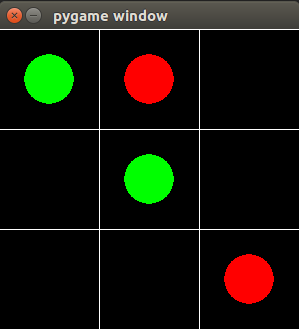
\includegraphics[width = 0.3\hsize]{ttt_example.png}
\caption{State of a tic-tac-toe game after 4 moves. The green player plays first (he is \texttt{player1}).}
\label{fig:ttt_ex}
\end{figure}

Here, we are the green player and we want to find a move such that we are sure to win in three moves.

\paragraph{Hypothesis space}

We use the following mode declaration:
\[ M=
\begin{Bmatrix} 
m1 :& \texttt{modeh(does(player1,\#move,5)).} \\ 
m2 :& \texttt{modeh(does(player1,\#move,7)).}\\
m3 :& \texttt{modeb(does(player2,\#move,6)).}\\
m4 :& \texttt{modeb(not does(player2,\#move,6)).}
\end{Bmatrix}
\]
%TODO : explain how a mode declaration works OR reference to an article to explain it

Moreover, we take the following hypothesis space:
\[ R_M=
\begin{Bmatrix}
\texttt{does(player1, X, 5).} \\ 
\texttt{does(player1, Z, 7) :-} & \texttt{does(player2, Y, 6).}\\
\texttt{does(player1, X, 7) :-}  & \texttt{not does(player2, Y, 6).}
\end{Bmatrix}
\]

So the top theory that we use for this example is:
\[ T=
\begin{Bmatrix}
\texttt{does(player1, X, 5) :-} & \texttt{legal(player1,X,5), rule((m1),(X)).} \\ 

\texttt{does(player1, Z, 7) :-} & \texttt{legal(player1, Z, 7), legal(player2, Y, 6), }\\ 
 & \texttt{does(player2, Y, 6), rule((m2,m3,2),(Z,Y)).} \\

\texttt{does(player1, X, 7) :-} & \texttt{legal(player1, X, 7), legal(player2, Y, 6), } \\
& \texttt{not does(player2, Y, 6), rule((m2,m4,2),(X,Y)).}
\end{Bmatrix}
\]
where we added the predicate \texttt{legal/3} to make the variables safe.

\bigskip

So now the hypothesis we want to learn with ILASP has the following form:
\[H=
\begin{Bmatrix}
\texttt{rule((m1),(\#move\_p1\_t0\_1)).}\\
\texttt{rule((m2,m3,2),(\#move\_p1\_t2\_1, \#move\_p2\_t1\_1))}.\\
\texttt{rule((m2,m4,2),(\#move\_p1\_t2\_2, \#move\_p2\_t1\_1))}.
\end{Bmatrix}
\]

\bigskip

We want $H$ to contain only one rule of each type: only one rule of the form\\ \texttt{rule((m1),(\#move\_p1\_t0\_1))} and so on... 
So we add some rules to make them unique:\newline
\texttt{rule1 :- rule((m1),(fill(coord(X,Y)))).}\\
\texttt{:- not rule1.}\\
\texttt{:- rule((m1),(fill(coord(X1,Y1)))), rule((m1),(fill(coord(X2,Y2)))), g(X1, Y1)< g(X2, Y2). }\\

\smallskip

The two first rules make \texttt{rule((m1),(\#move\_p1\_t0\_1))} appear at least once, and the last rule makes it appear at most once. We add similar rules for \texttt{rule((m2,m3,2), (\#move\_p1\_t2\_1, \#move\_p2\_t1\_1))} and \texttt{rule((m2,m4,2), (\#move\_p1\_t2\_2, \#move\_p2\_t1\_1))}.

\bigskip

Also, we added some constraints to reduce the computation time. For instance, if \texttt{rule((m1),(fill(coord(X,Y))))} is true, then \texttt{legal(player1,fill(coord(X,Y)),5)} must be true. So we add the following constraint:\newline
\texttt{:- rule((m1),(fill(coord(X,Y)))), not legal(player1,fill(coord(X,Y)),5).}

\bigskip

And if \texttt{rule((m2,m4,2),(fill(coord(X,Y)),fill(coord(Z,T))))} and \texttt{not does(player2, fill(coord(Z,T)), 6)} are true, then \texttt{legal(player1, fill(coord(X,Y)),7)} must be true unless \texttt{player2} plays in \texttt{coord(X,Y)} at time 6. Thus, we add the following constraint:\newline
\texttt{:- rule((m2,m4,2),(fill(coord(X,Y)),fill(coord(Z,T)))), not does(player2, fill(coord(Z,T)), 6),}
\texttt{ not legal(player1, fill(coord(X,Y)),7).}\newline
and we add this context-dependent example to the set of positive examples : \newline
$<<\{\texttt{wins(player2,8)}\},\emptyset>,\\ \{\texttt{:- rule((m2,m4,2),(fill(coord(X,Y)),fill(coord(Z,T)))),} \\ \texttt{not does(player2, fill(coord(X,Y)), 6).}\}>$
%TODO : change fonts to textt in partial interpretations

\smallskip

With this example, we are sure that there will be at least one answer set where \texttt{player2} plays in \texttt{coord(X,Y)}.


\paragraph{Declaring the examples}

First of all, we want the first player to win in two moves all the time. So there is no answer set that does not contain \texttt{wins(player1,8)}. Thus, we take : $E^-=\{<\emptyset,\{\texttt{wins(player1,8)}\}>\}$.

\bigskip

For the positive examples, we only need to take the one given in the previous paragraph. The \texttt{wins(player2,8)} in it is optional but it reduces the computation time from 11 seconds to 1 second.

\paragraph{Evaluation}

%TODO : to complete

\subsection{Finding a move in the middle of a game}

We are only able to look two moves ahead, so we cannot predict how to win a game if we are not very close to the end. It would be a good idea to define what a good state is (or to make ILASP learn it). And after that, it could be possible to choose a state at time $t$ that maximizes the chances of reaching a good state at time $t+2$.

\bigskip

For instance, if we consider the game represented in figure \ref{fig:graph_game}, where \texttt{player1} plays at times $t$ and $t+2$ and \texttt{player2} plays at time $t+1$. 

\smallskip

We want to maximize the probability of reaching a good state at $t+2$. So we choose $a(x)$ such that $\#\{b(y)|legal(b(y))\wedge\:\left( b(y) \implies \exists \:c(z) \:;\: legal(c(z)) \wedge good\_state(state\_c(z)) \right)\}$ is maximal, which is $a(1)$ in this example.

\begin{figure}[h]
\centering
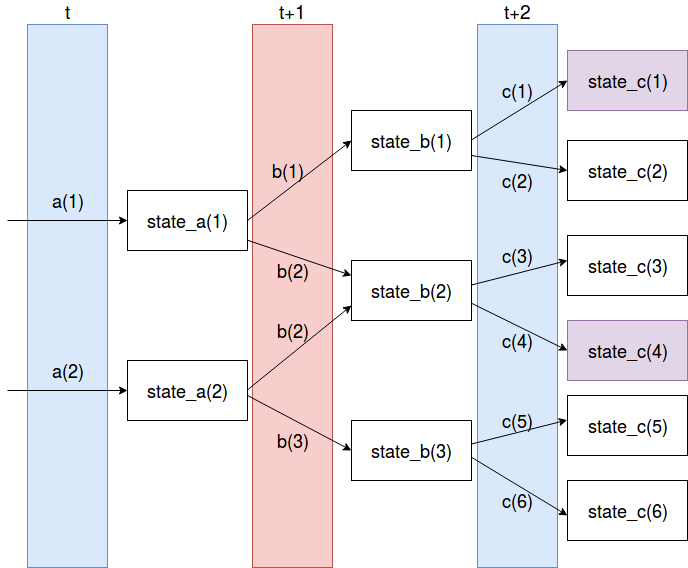
\includegraphics[width = 0.8\hsize]{graph_game.png}
\caption{Desription of a graph game with its states and the actions to perform to go from one state to another. The blue player (that plays at times $t$ and $t+2$) is \texttt{player1}. The states in purple are the good states.}
\label{fig:graph_game}
\end{figure}

\section{Second Method: recognize preferred patterns}




%% bibliography
\bibliographystyle{abbrv}
\bibliography{exemple}

\end{document}
